%
% ** SECTION 8 **
%

\begin{summary}
The coming decade will be an exciting time for cosmology. Before WFIRST launch,
major cosmological imaging surveys (KiDS, HSC, DES) and the DESI and PFS
spectroscopic surveys will significantly advance our current understanding.
WFIRST, Euclid and LSST  will then go further and survey the sky at optical and
infrared wavelengths, the  James Webb Space Telescope (JWST) and the Extremely
Large Telescopes (ELTs) will make very deep maps of the sky; eROSITA will survey
the X-ray sky; CMB-S4 will make a deep map of the millimeter sky; and the
Canadian Hydrogen Intensity Mapping Experiment (CHIME) and other radio surveys
will map the large-scale distribution of H$\,${\sc i}. One goal of our SIT is to
determine the analysis infrastructure and observations needed to achieve the
full potential of WFIRST in combination with these  surveys. This is best done
through a broad community effort that brings together scientists from these
complementary projects. For this purpose, we organized a first community
workshop focused on enabling the cosmological scientific synergies between
WFIRST and LSST.
\end{summary}

%Our SIT team is well-placed to do this, through team members' significant roles in a number of these projects and ties to the other major surveys.

%Our team will explore ways of maximizing the science return from these combined data sets. Our team members are playing significant roles in a number of these projects and have good ties to the other major surveys.

We started to actively engage the community to identify and pursue the key areas
where WFIRST and the concurrent projects will provide new opportunities to
mitigate systematics and enhance the combined cosmological science return. We
started a series of open community workshops to incorporate the interplay
between major planned surveys and WFIRST into the WFIRST strategy, to identify:
(i) pre-launch observations, (ii) how these external data sets affect the WFIRST
observing strategy (e.g., deep fields) and the instrument, and (iii) the
software needed (to be built post-CDR) for combining these data sets.

\paragraph*{First Community Workshop} The first of this meeting happened in
Pasadena in September 2016. It was focused on the synergies between the WFIRST
HLS Cosmology SIT and LSST Dark Energy Science Collaboration (DESC), both at the
science level but also at the implementation level. The meeting was co-organized
by Rachel Bean, Olivier Dor\'e, Steve Kahn and Jason Rhodes and was attended by
about 60 scientists from the two collaborations. The slides are available
\href{https://conference.ipac.caltech.edu/wfirst_lsst/}{here} and pictures can
be seen in Figure~\ref{fig:pic_workshop}. The conclusion of the lively and
productive workshop will be summarized in a white paper to be written shortly.

\begin{figure}
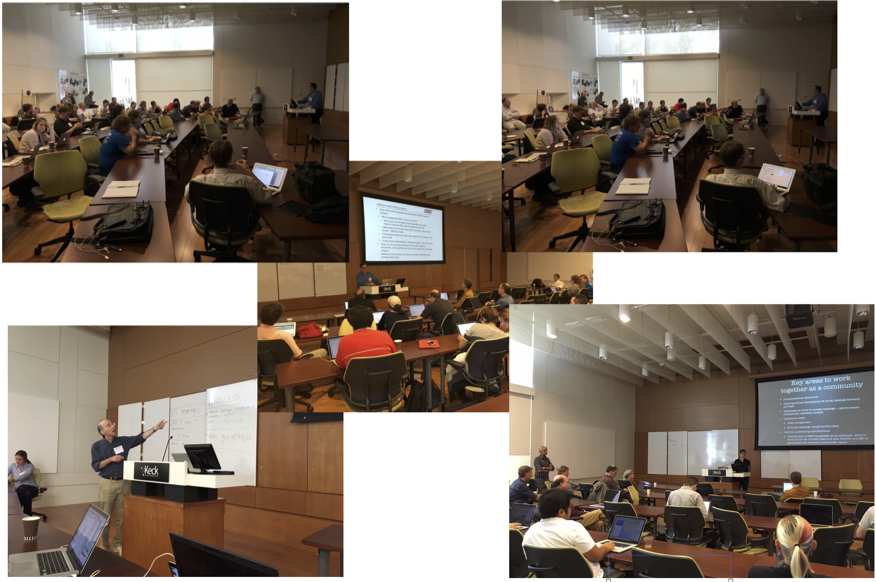
\includegraphics[width=\textwidth,angle=0]{Plots/pic_workshop.pdf}
\caption{\label{fig:pic_workshop}Pictures taken during the Pasadena WFIRST SIT - LSST DESC workshop on September 2016.}
\end{figure}

\paragraph*{Premise} The workshop was built on the premise that when considering
joint science return from LSST and WFIRST, \emph{the whole is greater than the
sum of the parts}, as already articulated in \citet{Jain:2015cpa}. In the
conclusion of the Jain et al. community white paper, it was articulated that the
scientific opportunity offered by the combination of data from LSST and WFIRST
(and Euclid) goes well beyond the science enabled by any one of the data sets
alone. The range in wavelength, angular resolution and redshift coverage that
these missions jointly span is remarkable. With major investments in LSST and
WFIRST (and partnership with ESA in Euclid), the US has an outstanding
scientific opportunity to carry out a combined analysis of these data sets. It
is imperative for us to seize it and, together with our European colleagues,
prepare for the defining cosmological pursuit of the 21st century.

As illustrated already in \S~\ref{sec:forecast}, the coming decade will be the
era of multi-probes/multi-survey science. The richer insights will come from
combining multiple probes (WL, GRS, GC) \emph{reliably}. If done properly,
multiple survey joint analysis will enable new calibration schemes (photo-$z$,
intrinsic alignment models, etc.) and new control of systematics (PSF effects,
contaminant control such as stars or interlopers).

\paragraph*{Joint Analysis} The main argument for conducting a single,
high-quality reference co-analysis exercise and carefully documenting the
results is the complexity and subtlety of systematics that define this
co-analysis. Falling back on many small efforts by different teams in selected
fields and for narrow goals will be inefficient, leading to significant
duplication of effort.  For much of the science, we will need to combine the
photometry across multiple wavelengths with varying spectral and spatial
resolution – a technical challenge. The joint analysis can be carried out in
ways that have different computational demands. The most technically demanding
joint analysis is to work with pixel level data of the entire area of overlap
between the surveys. Many of the goals of a joint analysis require such a
pixel-level analysis. If pixel-level joint analysis is not feasible,
catalog-level analysis can still be beneficial, say to obtain calibrations of
the lensing shear or the redshift distribution of galaxies. Hybrid efforts are
also potentially useful, for example using catalog level information from space
for deblending LSST galaxies, or using only a mutually agreed subset of the data
for calibration purposes. However the full benefits of jointly analyzing any two
of the surveys can be reaped only through pixel-level analysis \citep{Jain:2015cpa}.

\paragraph*{Possible Implementation} In the workshop, possible algorithmic
implementation of a joint analysis pipeline were discussed independently by
Peter Melchior and Michael Schneider. \citet{Melchior:2016asy} motivated the
need for complex galaxy morphology models and developed the relevant statistical
framework. For them, complex models become the norm. They are more flexible and properly
behaved. WFIRST benefits from LSST through color-morphology priors. LSST
benefits from sharp likelihood peaks in WFIRST bands. LSST benefits from WFIRST
through superior resolution. \citet{Schneider:2014rha} have developed a probabilistic
image reduction pipeline (forward modeling) motivated by challenges in
multi-epoch/multi-telescope combinations. They demonstrated improved shear
measurements for LSST using the HST Frontier field as a proxy for WFIRST.

\paragraph*{Enabling Synergies} It was recognized in the context of photo-$z$ for example, that
cooperation already exist to maximize utility and minimize duplication in
spectroscopic calibration samples. Capak and collaborators are building a public
calibration catalog for WFIRST and LSST \citep{Masters2017}. Also, relevant information for deep
surveys synchronization, is also discussed in this context and others (SNe,
shape calibration, grism calibration, guest observations). The detailed requirements for LSST + WFIRST photo-$z$ performance are however still to be articulated.

\paragraph*{Computing Needs} Large computing efforts are under way in LSST
(DESC) with multiple planned data challenges. Resources available for the scale
of simulations required (with possible exception of hydrodynamical simulations)
are secured. However, ressources needed for sharing simulations (e.g. Millennium
DB) and mock catalogs are required. They have historically greatly 
expanded the
use of simulations in a broad range of applications. A 100 TB to 1 PB scale
infrastructure simply does not exist and data transfer will be a challenge (10
days for 100 TB at 1 Gb). There is great opportunity for future collaborations
(e.g., joint mock catalogs) and investments. Opportunity for collaborations and
investments. As we will discuss in \S\ref{sec:tacs}, members of our team are leading and participating in a Tri-Agency Cosmological Simulations (TACS) dedicated to this issue.

\paragraph*{Ressources} As already discussed in \citet{Jain:2015cpa}, the resources required to achieve this additional
science are outside of what is currently budgeted for LSST by NSF and DOE, and
for WFIRST (or Euclid) by NASA. Funding for this science would most naturally
emerge from coordination among all agencies involved, and would be closely
orchestrated scientifically and programmatically to optimize science returns. A
possible model would be to identify members of the science teams of each project
who would work together on the joint analysis. The analysis team would ideally
be coupled with an experienced science center acting as a focal point for the
implementation, and simultaneously preparing the public release and documentation for broadest access by the community.

\paragraph*{Future Workshop} The second in our series of SIT community workshop
will happen in the fall 2017 in Pasadena, synchronized with a FSWG, and will
identify (and discuss the enabling of) scientific synergies between the HLS and
other major surveys across all wavelengths.
